% !TEX program = pdflatex
% SafeBoxForest — IROS 2025 Submission
% Compile: pdflatex → bibtex → pdflatex × 2
\documentclass[letterpaper, conference]{IEEEtran}

% ─── Packages ────────────────────────────────────────────────────────────────
\usepackage[utf8]{inputenc}
\usepackage[T1]{fontenc}
\usepackage{amsmath,amssymb,amsthm}
\usepackage{graphicx}
\usepackage{algorithmic}
\usepackage{algorithm}
\usepackage{booktabs}
\usepackage{multirow}
\usepackage{cite}
\usepackage{xcolor}
\usepackage{hyperref}
\usepackage{cleveref}
\usepackage{bm}
\usepackage{tabularx}
\usepackage{balance}   % balanced last-page columns
\usepackage{xspace}    % proper spacing after macros
\usepackage{microtype}  % microtypographic enhancements

% ─── IEEE / IROS margin compliance ──────────────────────────────────────────
% All margins 54pt; first-page extra 18pt added via \vspace in \title
\usepackage[letterpaper,
  top=54pt, bottom=54pt, left=54pt, right=54pt]{geometry}

% ─── Theorem environments ────────────────────────────────────────────────────
\newtheorem{theorem}{Theorem}
\newtheorem{definition}{Definition}
\newtheorem{remark}{Remark}
\newtheorem{proposition}{Proposition}
\newtheorem{assumption}{Assumption}

% ─── Custom commands ─────────────────────────────────────────────────────────
\newcommand{\Cfree}{\mathcal{C}_\text{free}}
\newcommand{\Cspace}{\mathcal{C}}
\newcommand{\AABB}{\text{AABB}}
\newcommand{\FK}{\text{FK}}
\newcommand{\SBF}{\text{SBF}}
\newcommand{\Real}{\mathbb{R}}
\newcommand{\calO}{\mathcal{O}}
\newcommand{\calA}{\mathcal{A}}
\newcommand{\calF}{\mathcal{F}}
\newcommand{\calR}{\mathcal{R}}
\newcommand{\bT}{\mathbf{T}}
\newcommand{\TODO}[1]{\textit{[Placeholder: #1]}}
\newcommand{\ie}{\textit{i.e.},\xspace}
\newcommand{\eg}{\textit{e.g.},\xspace}
\newcommand{\cf}{\textit{cf.}\@\xspace}
\newcommand{\etal}{\textit{et~al.}\@\xspace}
\DeclareMathOperator{\interior}{int}

% ==============================================================================
\begin{document}

\title{\vspace{18pt}SafeBoxForest: Rapid C-space Box Cover with\\
Lifelong Envelope Caching for GCS Planning}

\author{
\IEEEauthorblockN{TIAN, Yu and Ren, Hongliang$^{*}$}
\IEEEauthorblockA{Department of Electronic Engineering,
The Chinese University of Hong Kong,\\
Shatin, N.T., Hong Kong SAR, China\\
\{ty1997, hlren\}@ee.cuhk.edu.hk}
}
\maketitle

% ==============================================================================
% ABSTRACT
% ==============================================================================
\begin{abstract}
Graph of Convex Sets~(GCS) is a state-of-the-art framework for
convex-optimization-based motion planning that requires convex
free-space regions as input.
Existing IRIS-family region generators either lack collision-safety
certificates or require minutes per region, and none supports
incremental updates when the scene changes.
We present \emph{SafeBoxForest}~(SBF), a certified region generator
for GCS.
SBF introduces a \emph{Lifelong Envelope Cache Tree}~(LECT) that
maps C-space boxes to certified workspace
axis-aligned bounding box~(AABB) envelopes via
\emph{interval forward kinematics}~(FK).
Because envelopes depend only on robot kinematics,
they are computed once on demand and cached for the robot's lifetime.
Given an obstacle scene, SBF queries the LECT and grows a
collision-free box forest via wavefront expansion.
Greedy coarsening merges fine boxes into larger certified regions
that map directly to a GCS graph.
When obstacles change, only the affected boxes are regrown.
On a 7-DOF KUKA IIWA14 manipulator, SBF generates certified regions
$86$--$123\times$ faster than IRIS-NP with a 98\% GCS planning
success rate.
Incremental regrowth takes just $7$\,ms ($1/150$ of a cold rebuild).
\end{abstract}

% ==============================================================================
% I. INTRODUCTION
% ==============================================================================
\section{Introduction}\label{sec:intro}

Graph of Convex Sets~(GCS)~\cite{marcucci2024motion}
formulates motion planning as optimization over a graph of convex
free-space regions.
It produces high-quality trajectories via convex relaxation.
However, planning quality depends on the upstream \emph{region generation}
step: how to quickly produce certified collision-free convex regions.
In assembly lines and human--robot collaboration, obstacles change
frequently while the robot remains the same, so region generators
must support incremental updates rather than full rebuilds.
Existing IRIS-family methods do not meet this need.
IRIS-NP~\cite{petersen2023growing} lacks formal collision-safety
certificates.
C-IRIS~\cite{werner2024certified} provides certificates but requires
minutes per region.
No existing method supports persistence or cross-scene reuse.
SBF targets applications where formal collision-free guarantees are
mandatory (subject to the geometry-enclosure assumption stated in
\cref{sec:ifk}).
It trades individual-region volume for certified safety and
orders-of-magnitude speed advantage.

For a serial manipulator, given a C-space box, one can compute a
workspace AABB for each link that encloses the link geometry over all
configurations in that box.
We call this AABB a \emph{link-AABB envelope}
(\cref{fig:overview}a--b).
The mapping from C-space box to link-AABB vector depends \emph{only}
on robot kinematics, \emph{not} on obstacles.
This observation enables a lazy caching design.
A KD-tree called the LECT lazily
computes and caches AABB envelopes for C-space cells on demand.
Each envelope is computed once and reused permanently across all scenes.
Given a specific scene, SBF queries the LECT for cached AABBs and
grows a collision-free box forest.
The forest maps directly to a GCS graph.
Based on this observation, SBF makes the following contributions:

\begin{enumerate}
\item \textbf{Certified lifelong caching}
  (\cref{sec:ifk,sec:lect}):
  The LECT maps C-space boxes to
  certified workspace AABB envelopes via interval-FK.
  Each envelope is computed on demand and cached permanently.
  Because envelopes depend only on robot kinematics, the cache is
  reusable across all scenes for the robot's lifetime.

\item \textbf{Rapid certified region generation}
  (\cref{sec:sbf_construction,sec:sbf_forest,sec:coarsen}):
  Starting from seed configurations, boxes expand outward via
 wavefront expansion.
  Bridge paving connects isolated components.
  A tree-cached two-stage hull check then merges thousands of fine
  boxes into hundreds of certified regions that map directly to a
  GCS graph.

\item \textbf{Strong cross-scene reusability}
  (\cref{sec:incremental}):
  When obstacles change, targeted regrowth repairs only the affected
  boxes, reducing update time from seconds to milliseconds.
\end{enumerate}
Comprehensive experiments on a 7-DOF KUKA IIWA14 manipulator
(\cref{sec:experiments}) validate SBF's region-generation efficiency,
end-to-end GCS planning performance, and incremental-update
efficiency under obstacle perturbation.

\begin{figure*}[t]
\centering
\begin{tabular}{@{}c@{\hspace{4pt}}c@{\hspace{4pt}}c@{}}
\includegraphics[width=0.32\textwidth]{fig/1-1.png} &
\includegraphics[width=0.32\textwidth]{fig/1-3.png} &
\includegraphics[width=0.32\textwidth]{fig/1-5.png} \\
{\footnotesize (a) C-space SBF \& box $Q$} &
{\footnotesize (c) C-space path} &
{\footnotesize (e) Invalidated boxes} \\[4pt]
\includegraphics[width=0.32\textwidth]{fig/1-2.png} &
\includegraphics[width=0.32\textwidth]{fig/1-4.png} &
\includegraphics[width=0.32\textwidth]{fig/1-6.png} \\
{\footnotesize (b) Workspace AABBs of $Q$} &
{\footnotesize (d) Workspace path} &
{\footnotesize (f) After regrowth} \\
\end{tabular}
\caption{SBF visualization on a planar 2-link manipulator.
  (a,\,b)~Certified box forest in C-space and the workspace AABB envelopes of highlighted box~$Q$.
  (c,\,d)~GCS planned path through the coarsened box forest in C-space and the corresponding workspace trajectory.
  (e,\,f)~After a new obstacle is added, invalidated boxes (red) are identified and targeted regrowth repairs the region.}
\label{fig:overview}
\end{figure*}

% ==============================================================================
% II. RELATED WORK
% ==============================================================================
\section{Related Work}\label{sec:related}



\subsection{GCS Planning and Region Generation}

GCS~\cite{marcucci2024motion} casts motion planning as a mixed-integer convex
program over a graph of convex sets.
Tight convex relaxations yield globally optimal trajectories.
IRIS~\cite{deits2015computing} alternates between inscribed ellipsoids and
separating hyperplanes in workspace but does not directly produce C-space
regions.
IRIS-NP~\cite{petersen2023growing} grows C-space polytopes via nonlinear
seed-growing, achieving high volume but without formal collision-safety
certificates.
IRIS-ZO and IRIS-NP2~\cite{werner2024faster} apply zeroth-order and improved
nonlinear optimization to accelerate region generation, yet remain
non-certified.
C-IRIS~\cite{werner2024certified} provides sum-of-squares~(SOS)
polynomial certificates but requires minutes per region in
high-dimensional settings.
No existing method supports persistence or cross-scene reuse.

\subsection{C-space Decomposition and Cell Methods}

Exact cell decomposition~\cite{schwartz1983piano} is theoretically complete
but intractable in high dimensions.
Approximate cell decomposition~\cite{zhu1991new} employs octree/KD-tree
recursive splitting but lacks safety certification.
Approximate convex decomposition~\cite{lien2008approximate} primarily targets
workspace geometry and has not been extended to C-space certification.
SBF bridges the gap between approximate decomposition and certified safety
by combining interval-FK certificates with hierarchical cell refinement.

\subsection{Interval Arithmetic in Robotics}

Interval analysis provides rigorous enclosures of function
ranges~\cite{moore2009introduction,jaulin2001applied}.
Interval-FK has been used for workspace reachability
analysis~\cite{merlet2004solving} and parallel robot
calibration~\cite{daney2006interval}.
To the best of our knowledge, SBF is the first system to apply
interval-FK for C-space region certification in the context of GCS
planning.

\subsection{Sampling-Based Motion Planning}

Rapidly-exploring Random Tree~(RRT)~\cite{lavalle1998rapidly} grows a search tree by repeatedly
sampling a random configuration and extending the nearest node toward
it.
RRT-Connect~\cite{kuffner2000rrt} accelerates convergence by growing
two trees from start and goal simultaneously.
RRT$^*$~\cite{karaman2011sampling} adds asymptotic optimality via
rewiring.
All RRT-family planners explore C-space with point samples.
They produce a tree of configurations, not convex regions.
SBF's forest growth borrows the wavefront expansion idea from RRT:
a seed configuration is analogous to an RRT root, and face sampling
extends the frontier outward.
The key difference is that SBF expands certified \emph{boxes}
rather than point samples.
Each box carries an interval-FK safety certificate and directly
serves as a GCS node.

\subsection{Multi-Query and Persistent Planning}

Probabilistic Roadmap~(PRM)~\cite{kavraki1996probabilistic} builds a persistent roadmap that
supports multi-query planning but provides neither convex regions nor
collision-safety certificates.
Experience Graphs~\cite{phillips2012experience} reuse historical paths but
do not generate free-space regions.
SBF uniquely combines certified convex region generation, persistence, and
incremental updates in a single framework.

% ==============================================================================
% III. LIFELONG CERTIFIED ENVELOPE CACHE TREE
% ==============================================================================
\section{Lifelong Certified Envelope Cache Tree}
\label{sec:certification}

This section first presents the certification problem and
interval-FK, which computes certified AABB envelopes for C-space boxes.
The LECT then organizes these envelopes in a
lazy KD-tree cache that is scene-independent and reusable across the
robot's lifetime.

% ──── III-A. Problem Formulation ─────────────────────────────────────────────
\subsection{Certified Envelope via Interval-FK}\label{sec:ifk}

Consider a $D$-DOF serial manipulator with $L$ collision-relevant links.
Given a C-space box $B \subset \Real^D$ and a set of obstacle
AABBs $\calO$ in the workspace, the goal is to determine whether
$B \subseteq \Cfree$, \ie the robot is collision-free for every
$\bm{q} \in B$.

\emph{Link-AABB envelope.}
For link~$\ell$ and C-space box~$B$, the \emph{link-AABB envelope}
$\AABB_\ell(B)$ is a workspace AABB satisfying
\begin{equation}\label{eq:envelope}
  \AABB_\ell(B) \supseteq \bigcup_{\bm{q} \in B}
    \mathrm{geom}_\ell\bigl(\FK(\bm{q})\bigr).
\end{equation}
Each link is modeled as a line segment connecting two adjacent joint
origins, inflated by a collision radius~$r_\ell$ that conservatively
encloses the true mesh geometry.
We assume that this inflated capsule always contains the true link
geometry (\cref{asm:geom}).

\begin{assumption}[Geometry Enclosure]\label{asm:geom}
For each link~$\ell$ and all $\bm{q} \in \Cspace$,
$\mathrm{geom}_\ell\bigl(\FK(\bm{q})\bigr) \subseteq
 \mathrm{capsule}_\ell\bigl(\FK(\bm{q}),\, r_\ell\bigr)$.
\end{assumption}

Under \cref{asm:geom}, the envelope~\eqref{eq:envelope} contains
every link's true geometry over the entire box~$B$.
If $\AABB_\ell(B) \cap O_j = \emptyset$ for all links~$\ell$ and
obstacles~$O_j$, then $B \subseteq \Cfree$.
This is a conservative sufficient condition: intersection does
\emph{not} imply collision, only that the box cannot be certified at
this granularity.

\emph{Computing the envelope via interval-FK.}
The standard DH transformation matrix $\bT_i(\theta_i)$ maps frame $i$
to frame $i{-}1$.
Substituting interval trigonometric functions for joint-angle intervals
yields an interval matrix $[\bT_i]$.
The forward kinematics to frame $k$ is obtained by sequential interval
matrix multiplication:
\begin{equation}\label{eq:chain}
  [\bT^{0:k}] = [\bT^{0:k-1}] \otimes [\bT_k],
\end{equation}
where $\otimes$ denotes interval matrix multiplication.
The AABB for link~$\ell$ is extracted from the translation vectors of
$[\bT^{0:\ell-1}]$ and $[\bT^{0:\ell}]$ (representing the two
endpoints), then inflated by~$r_\ell$.

\emph{Certified conservatism.}
By the inclusion-monotonicity property of interval
arithmetic~\cite[Theorem~4.1]{moore2009introduction}, interval-FK provides a
provably conservative AABB enclosure.
Chain multiplication may introduce over-approximation due to the
dependency problem (the \emph{wrapping effect}).
This affects the \emph{tightness} of the enclosure but not its
\emph{soundness}.

\emph{Complexity.}
Certifying a single box requires computing the interval transform
chain once ($D$ interval matrix multiplications of fixed $4{\times}4$
size), then extracting~$L$ link AABBs.
With prefix sharing, the total cost is $O(D + L)$.

% ──── III-B. Lifelong Envelope Cache Tree ────────────────────────────────────
\subsection{Lifelong Envelope Cache Tree (LECT)}\label{sec:lect}

The LECT is a KD-tree over C-space that organizes and caches the AABB
envelopes computed by interval-FK.

\emph{Structure.}
The root covers the full configuration space $\Cspace$.
Each internal node bisects one dimension.
Each node~$v$ stores a C-space box $B_v$ and its cached envelope vector
$\calA(B_v) = (\AABB_1(B_v),\ldots,\AABB_L(B_v))$.

\emph{Lazy growth.}
The LECT starts with a coarse root node covering $\Cspace$.
Nodes are split on demand when FFB queries (\cref{sec:sbf_construction})
require finer granularity.
A configurable maximum depth bounds the finest resolution.
Deeper splits produce smaller C-space boxes with tighter AABB envelopes.

\emph{FK prefix reuse.}
When a LECT node splits along dimension~$d$, the interval transform
chain $[\bT^{0:d-1}]$ for joints $1,\ldots,d{-}1$ is unchanged.
Only $[\bT^{d:D}]$ needs recomputation.
This saves approximately 43\% of computation on average (measured on
IIWA14 7-DOF).

\emph{Lifelong reuse.}
Each node's AABB envelope is computed once by interval-FK and cached permanently.
Because the envelope depends only on robot kinematics, a given
C-space box's AABB never changes across scenes.
The same LECT is reusable for the lifetime of a given robot.

\emph{Persistence.}
The LECT supports lightweight disk I/O: nodes are lazy-loaded on first
access and incrementally appended via mmap.
After warm start, the FK phase takes $<\!1$\,ms.
The bottleneck shifts entirely to collision detection.

% ──── III-C. Subdivision Enhancements ────────────────────────────────────────
\subsection{Subdivision Enhancements}\label{sec:subdivision}

Both subdivision techniques below are orthogonally applicable within the
interval-FK pipeline; they trade additional computation time for tighter
certified envelopes.

\emph{Link subdivision.}
A long link's AABB can be excessively large.
Splitting link~$\ell$ into $n$ equal segments along its local frame and
computing AABBs independently tightens the envelope.
Each sub-segment AABB is obtained by linearly interpolating the two
endpoint positions already available from the FK chain; no additional
FK evaluation is required.
The only overhead is $n{-}1$ extra AABB extractions per link, which
increases the number of AABB--obstacle tests in collision detection
but adds negligible FK cost.
Certification is preserved because each sub-segment AABB encloses
the corresponding portion of the link geometry.

\emph{C-space box subdivision.}
Bisecting $B$ along a dimension into $B_1,B_2$ and computing AABBs
separately yields tighter enclosures.
Recursive $k$-level subdivision produces $2^k$ sub-boxes.
Under interval-FK, sub-boxes share prefix transforms and \emph{certification is
preserved}
($\bigcup_i \AABB_\ell(B_i) \subseteq \AABB_\ell(B)$ but tighter).

Both subdivision techniques compose orthogonally with each other.
Thanks to interval-FK computation sharing (prefix-chain reuse), time overhead
grows sub-linearly while tightness improves significantly.


% ==============================================================================
% IV. SAFEBOXFOREST
% ==============================================================================
\section{SafeBoxForest: Growth, Coarsening, and GCS Integration}
\label{sec:sbf}

Given a specific obstacle scene, SBF grows a forest of certified
collision-free boxes on top of the LECT cache.
The growth process resembles RRT: starting from seed configurations,
boxes expand outward via face sampling.
Greedy coarsening then merges fine boxes into larger regions.
The resulting forest maps directly to a GCS graph.

% ──── IV-A. Forest Growth ────────────────────────────────────────────────────
\subsection{RRT-like Forest Growth}\label{sec:sbf_forest}

The construction procedure is given in \cref{alg:sbf}.
Each box is obtained by calling \emph{Find Free Box}~(FFB,
\cref{sec:sbf_construction}), which performs a top-down LECT search from
a seed configuration.

\begin{algorithm}[t]
\caption{SafeBoxForest Construction}\label{alg:sbf}
\footnotesize
\begin{algorithmic}[1]
\REQUIRE Robot~$R$, obstacles~$\calO$, $\bm{q}_\text{start}$, $\bm{q}_\text{goal}$,
  max boxes $N_{\max}$, random seeds $N_{\text{rand}}$
\ENSURE SafeBoxForest~$\calF$, GCS graph~$G$
\STATE Initialize LECT~$T$ (load from disk if available)
\STATE $B_s \leftarrow \text{FFB}(T, \bm{q}_\text{start}, \calO)$;\;
       $B_g \leftarrow \text{FFB}(T, \bm{q}_\text{goal}, \calO)$
\STATE $Q \leftarrow \{B_s, B_g\}$;\;
       $\calF \leftarrow \{B_s, B_g\}$
\WHILE{$|\calF| < N_{\max}$ \AND $Q \neq \emptyset$}
  \STATE $B \leftarrow \text{dequeue}(Q)$
  \FORALL{face $f \in \partial B$}
    \STATE $\bm{q}_\text{seed} \leftarrow \text{sample\_outside\_face}(f, \epsilon)$
    \IF{goal\_bias()}
      \STATE $\bm{q}_\text{seed} \leftarrow \text{perturb\_toward}(\bm{q}_\text{seed}, \bm{q}_\text{goal})$
    \ENDIF
    \STATE $B_\text{new} \leftarrow \text{FFB}(T, \bm{q}_\text{seed}, \calO)$
    \IF{$B_\text{new} \neq \emptyset$ \AND $B_\text{new} \notin \calF$}
      \STATE $\calF \leftarrow \calF \cup \{B_\text{new}\}$;\;
             $Q \leftarrow Q \cup \{B_\text{new}\}$
    \ENDIF
  \ENDFOR
\ENDWHILE
\STATE \COMMENT{Free Interval Weighted Sampling}
\FOR{$i=1$ \TO $N_{\text{rand}}$}
  \STATE $\bm{q}_\text{seed} \leftarrow \text{sample\_free\_interval\_weighted}(\calF)$
  \STATE $B_\text{new} \leftarrow \text{FFB}(T, \bm{q}_\text{seed}, \calO)$
  \IF{$B_\text{new} \neq \emptyset$}
    \STATE $\calF \leftarrow \calF \cup \{B_\text{new}\}$
  \ENDIF
\ENDFOR
\STATE \COMMENT{Bridge Paving}
\STATE $\mathcal{C} \leftarrow \text{connected\_components}(\calF)$
\FORALL{pair $(C_i,C_j) \in \mathcal{C} \times \mathcal{C}$}
  \STATE $\text{bridge\_paving}(T, C_i, C_j, \calO, \calF)$
\ENDFOR
\STATE $\calF \leftarrow \text{greedy\_coarsen}(\calF, T, N_\text{target})$
  \COMMENT{tree-cached hull check (\cref{sec:coarsen})}
\STATE $G \leftarrow \text{build\_adjacency}(\calF)$
\STATE $\text{save\_LECT}(T)$
\RETURN $\calF, G$
\end{algorithmic}
\end{algorithm}

\emph{Seed strategies.}
The growth process is analogous to RRT~\cite{lavalle1998rapidly}: boxes
expand outward from seed configurations, exploring free C-space
incrementally.
\emph{BFS wavefront} (lines~4--14): starting from $B_s$ and $B_g$, boxes
expand outward via $\epsilon$-offset face sampling.
With probability $p_\text{goal}=0.1$, the seed is perturbed toward
$\bm{q}_\text{goal}$ to accelerate goal-directed expansion
(analogous to RRT goal bias).
\emph{Free-interval weighting} (lines~16--19): sampling weighted by
per-dimension uncovered interval length fills coverage gaps.
\emph{Bridge paving} (lines~21--23): isolated connected components are
bridged in three steps.
First, a \emph{dry-run FFB} probes whether a candidate seed between two
components can yield a free box.
Then, an \emph{overlap check} ensures the new box does not violate~I1.
Finally, a \emph{formal FFB} inserts the box into $\calF$.
If direct bridging fails, an internal RRT-Connect~\cite{kuffner2000rrt}
finds a collision-free path between the components.
Additional boxes are paved along this path to restore connectivity.

% ──── IV-B. Find Free Box ────────────────────────────────────────────────────
\subsection{Find Free Box (FFB)}\label{sec:sbf_construction}

FFB is the core subroutine called by each expansion step in
\cref{alg:sbf}.
Given a seed configuration $\bm{q}_\text{seed}$, it performs a top-down
search in the LECT:
\begin{enumerate}
\item If node $B_v$ is collision-free $\to$ \emph{promotion}: return $B_v$
  (largest collision-free ancestor).
\item If collision $\to$ \emph{split}: bisect along the widest dimension,
  recurse into the child containing $\bm{q}_\text{seed}$.
\item At minimum-granularity leaf $\to$ return $\emptyset$ (mark as occupied).
\end{enumerate}
FFB reuses the LECT's cached AABBs for collision checking.
New nodes created during splitting are cached for future use.

\emph{Active split dimensions.}
Dimensions that do not affect any collision-relevant link geometry
are automatically excluded, reducing unnecessary splits.
For instance, if the last joint induces only a rotation about the link's
symmetry axis so that the link AABB remains invariant, that dimension
can be skipped.

\emph{Resolution completeness.}
If a collision-free path has $\ell_\infty$-clearance $\geq \delta$ and
the LECT leaf size satisfies $\delta_{\min} \leq \delta/2$, FFB
certifies a face-adjacent box chain covering the path (provided the
wrapping effect does not cause false rejection at leaf resolution).
SBF is therefore resolution-complete for paths of sufficient
clearance; $\delta_{\min}$ controls the resolution.

% ──── IV-C. Incremental Update ───────────────────────────────────────────────
\subsection{Incremental Update}\label{sec:incremental}

When the obstacle set changes from $\calO$ to $\calO'$, IRIS-family methods
cannot pinpoint invalidated regions and must fully reconstruct at cost
$O(N \cdot T_\text{IRIS})$.
SBF can precisely identify and surgically repair affected boxes via
a three-step \emph{targeted regrowth} procedure:
\begin{enumerate}
\item \textbf{Invalidate}: construct a single-obstacle collision checker
  for each changed obstacle and test every box's cached link AABBs
  against it, collecting the invalidated set~$\calF_\text{inv}$.
  Cost: $O(|\calF| \cdot L)$ per changed obstacle.
\item \textbf{Remove}: delete $\calF_\text{inv}$ from $\calF$ and the
  adjacency graph~$G$; \texttt{remove\_boxes} automatically cleans
  adjacency edges in both directions.
\item \textbf{Targeted regrow}: use the LECT's
  \texttt{sample\_unoccupied\_seed()} to draw seeds from depleted
  (unoccupied) tree regions.
  These regions are precisely the areas vacated by removed boxes.
  Each seed undergoes FFB, promotion, and
  \texttt{add\_box\_direct} ($O(N)$ incremental adjacency).
  This bypasses the full construction pipeline (wavefront, random fill,
  coarsening, global adjacency rebuild).
  The target count is $n_\text{target} = 2|\calF_\text{inv}|$.
\end{enumerate}
Because targeted regrow skips all heavyweight stages, its cost is
proportional to the number of invalidated boxes rather than the total
forest size.
Typical single-obstacle perturbations require only $1/150$ of
cold-rebuild time (\cref{tab:exp3}).

% ──── IV-D. Greedy Coarsening ─────────────────────────────────────────────
\subsection{Tree-Cached Greedy Coarsening}\label{sec:coarsen}

The BFS wavefront and random fill stages typically produce thousands of
fine-grained boxes (\eg ${\sim}2{,}000$ for the IIWA14 combined scene).
Greedy coarsening iteratively merges adjacent box pairs until a
target count $N_\text{target}$ is reached, preserving collision-safety
certificates (\cref{alg:coarsen}).

\begin{algorithm}[t]
\caption{Tree-Cached Greedy Coarsening}\label{alg:coarsen}
\footnotesize
\begin{algorithmic}[1]
\REQUIRE Forest~$\calF$, collision checker, target~$N_\text{target}$,
  HierAABBTree~$T$, FK budget per round~$B_\text{fk}$
\ENSURE Coarsened forest~$\calF'$
\REPEAT
  \STATE Rebuild face-adjacency pairs of $\calF$
  \FOR{each adjacent pair $(A,B)$}
    \STATE $H \leftarrow \text{bbox}(A \cup B)$;\;
           $s \leftarrow \mathrm{vol}(H)/(\mathrm{vol}(A)+\mathrm{vol}(B))$
    \IF{$s \leq 50$}
      \STATE Add $(s, A, B, H)$ to candidates
    \ENDIF
  \ENDFOR
  \STATE Sort candidates by $s$ ascending
  \STATE $\text{fk\_count} \leftarrow 0$
  \FOR{each candidate $(A, B, H)$ in order}
    \IF{$|\calF| \leq N_\text{target}$}
      \STATE \textbf{break}
    \ENDIF
    \STATE $\text{safe} \leftarrow \neg\;\texttt{check\_box}(H)$
      \COMMENT{Stage 1: fast interval-FK}
    \IF{$\neg\text{safe}$ \AND $T \neq \text{null}$
        \AND $\text{fk\_count} < B_\text{fk}$}
      \STATE $\text{safe} \leftarrow T.\texttt{check\_hull\_safe}(H, A, B)$
        \COMMENT{Stage 2}
    \ENDIF
    \IF{safe}
      \STATE Merge $A, B$ into $H$ in $\calF$
    \ENDIF
  \ENDFOR
\UNTIL{no merges this round \OR max rounds reached}
\RETURN $\calF$
\end{algorithmic}
\end{algorithm}

Each hull candidate~$H$ is certified by a two-stage check.
Stage~1 runs a fast full-box interval-FK test (${\sim}\mu$s).
Stage~2, invoked only when Stage~1 fails, traverses the LECT to
verify only the gap region $H \setminus (A \cup B)$, reusing cached
AABBs and skipping nodes already covered by $A$ or $B$.
An FK-call budget per round (default 2{,}000) prevents cost explosion.
Tree-cached coarsening reduces box count from 1{,}042 to 457
(56\% further reduction) while increasing coverage from 25.8\% to
30.5\%, all within 1\,s.

% ──── IV-E. GCS Graph Generation ─────────────────────────────────────────────
\subsection{GCS Graph Generation}\label{sec:gcs_graph}

The coarsened forest $\calF = \{B_1,\ldots,B_N\}$ is mapped to a
GCS graph $G=(V,E)$ as follows.

\emph{Nodes.}
Each box $B_i = [\bm{l}_i,\,\bm{u}_i]$ is an axis-aligned
hyperrectangle, representable as a HPolyhedron with $2D$ halfplane
constraints ($\bm{l}_i \leq \bm{q} \leq \bm{u}_i$).
This representation requires no vertex enumeration or convex-hull
computation.

\emph{Edges.}
Two boxes $B_i,B_j$ are face-adjacent iff they share a
$(D{-}1)$-dimensional face: one dimension $d$ satisfies
$u_i^d = l_j^d$ (or vice versa) and all other dimensions overlap.
Each edge carries a continuity constraint ensuring the trajectory
is continuous across the shared face.

\emph{Source and target.}
The boxes containing $\bm{q}_\text{start}$ and $\bm{q}_\text{goal}$
serve as source and target nodes.
Boxes are non-overlapping
($\interior(B_i) \cap \interior(B_j) = \emptyset$ for $i \neq j$),
so each query point belongs to at most one box.

% ==============================================================================
% V. EXPERIMENTS
% ==============================================================================
\section{Experiments}\label{sec:experiments}

All experiments use a KUKA IIWA14 7-DOF manipulator
($D{=}7$, $L{=}7$) on Ubuntu~22.04 (Intel Core~i7).
SBF is implemented in C++ with pybind11 bindings;
all GCS methods use Drake~\cite{tedrake2019drake} with
Mosek~\cite{mosek2024} as the SOCP backend.
The test scene is the combined Marcucci
benchmark~\cite{marcucci2024motion} with 16 AABB obstacles
(shelves, bins, and a table; \cref{fig:exp2_viz}).
Five query pairs form a cyclic tour through five milestone
configurations.
We compare \textbf{SBF-GCS}~(ours) with \textbf{IRIS-NP-GCS},
both feeding into the same GCS-SOCP solver.
C-IRIS~\cite{werner2024certified} is excluded because a single
region requires 2--5\,min in 7-DOF settings.
Both methods use 8~Marcucci milestone configurations as seeds;
SBF repeats each setup 10~times (seed~0--9).
To validate certification, we sample $10^4$~configurations per box
and check against FCL~\cite{pan2012fcl}; no collision is detected.

% ──── Exp 1 ──────────────────────────────────────────────────────────────────
\subsection{Region Generation Efficiency}\label{sec:exp1}

This experiment directly compares the core region-generation capability of
SBF versus IRIS-NP, which is the current standard region generator for GCS
planning.

\emph{Design.}
Both methods are run to completion on the combined scene with a
reduced planning subspace (0.033\% of the original C-space volume)
derived from the milestone configurations with 0.3\,rad margin.
IRIS-NP uses 8 manually chosen seed configurations
from~\cite{marcucci2024motion} and Drake's \texttt{IrisNp}
implementation with \texttt{iteration\_limit}$\,{=}\,$10.
SBF uses the same 8~milestone configurations as BFS root seeds
(box budget~1{,}000; random fill~200; $\delta_{\min}{=}0.02$\,rad;
coarsen target~200; split\_depth~1; FK budget~2{,}000)
and is evaluated under two conditions:
\emph{cold} (no LECT; tree built from scratch) and
\emph{warm} (LECT loaded from a previous run),
demonstrating the cross-seed stability and cache reuse benefit.
Coverage is estimated via Monte Carlo sampling
($10^5$ points evaluated purely within the 0.033\% relevant subspace, independent RNG seed).

\begin{table}[t]
\centering
\caption{Region generation on the combined scene (SBF: mean$\pm$std, 10 seeds).}
\label{tab:exp1}
\footnotesize
\begin{tabular}{@{}lcccr@{}}
\toprule
Method & \#\,Regions & Coverage & Time & Speedup \\
\midrule
SBF cold  & $892{\pm}59$ & (23.6 $\pm$ 1.8)\% & \textbf{1.05\,s}${\pm}$0.27 & \textbf{86$\times$} \\
SBF warm  & $850{\pm}33$ & (24.5 $\pm$ 1.7)\% & \textbf{0.73\,s}${\pm}$0.29 & \textbf{123$\times$} \\
\midrule
IRIS-NP$^\dagger$ & 8 & \textbf{60.0\%} & 89.95\,s & 1$\times$ \\
\bottomrule
\end{tabular}
\\[2pt]
{\scriptsize $^\dagger$\,8 seed points, Drake IrisNp, \texttt{iteration\_limit}$\,{=}\,$10.\\
Regions = after greedy coarsening.  Speedup vs.\ IRIS-NP.}
\end{table}



\emph{Analysis.}
IRIS-NP produces 8 high-volume polytopes (18.23 $\text{rad}^7$ total volume)
achieving 60.0\% free-space coverage, but requires 90\,s (over
11\,s per region).
SBF cold generates ${\sim}$2{,}700 certified boxes and coarsens them to
${\sim}$892 in a total of 1.05\,s (\textbf{86$\times$ faster} than IRIS-NP)
with 23.6\% coverage.
SBF warm loads a previously cached LECT from disk.
It achieves 24.5\% coverage with ${\sim}$850 post-coarsening boxes in
0.73\,s (\textbf{123$\times$ faster}), a \textbf{1.44$\times$ speedup}
over cold start.
The LECT warm start reduces build time by eliminating redundant FK
computations.
Cached AABBs enable the coarsening stage's tree-traversal to verify
more hull candidates without recomputing forward kinematics.
While IRIS-NP's individual polytopes are volumetrically larger,
they lack collision-safety certificates;
each SBF box carries a formal interval-FK certificate.
The coverage gap reflects the conservatism of hyperrectangular envelopes
(the wrapping effect).
Importantly, this lower \emph{global} coverage does not preclude
effective planning.
\Cref{fig:exp2} confirms that SBF's densely packed boxes concentrate
coverage along planning-relevant corridors,
achieving a 98\% success rate with paths only 11\% longer on average.
Moreover, SBF's persistent cache enables instantaneous reuse across
scenes (\cref{tab:exp3}).
IRIS-NP cannot provide this capability
(\cref{tab:exp1}).

\emph{Speed--coverage tradeoff.}
SBF's lower global coverage is not an inherent ceiling:
increasing the box budget, subdivision depth, or random-fill rounds
would raise coverage at the cost of longer build time.
SBF deliberately prioritizes speed---completing region generation
two orders of magnitude faster than IRIS-NP---while
BFS wavefront seeding concentrates certified boxes along
planning-relevant corridors, preserving a competitive success rate
(\cref{fig:exp2}).



% ──── Exp 2 ──────────────────────────────────────────────────────────────────
\subsection{End-to-End GCS Planning Performance}\label{sec:exp2}

This experiment evaluates whether SBF-generated regions translate into
competitive downstream planning.

\emph{Metrics.}
Per-pair planning success rate~(\%);
GCS solver time;
path length (C-space $L_2$).

\begin{figure}[t]
\centering
\includegraphics[width=\columnwidth]{fig/exp2.png}
\caption{3-D workspace visualization of SBF-GCS planned trajectories
  on the combined scene (seed~0).
  Trajectory colors: Task~1 blue, 2 yellow, 3 green, 4 red, 5 purple.}
\label{fig:exp2_viz}
\end{figure}

\begin{figure}[t]
\centering
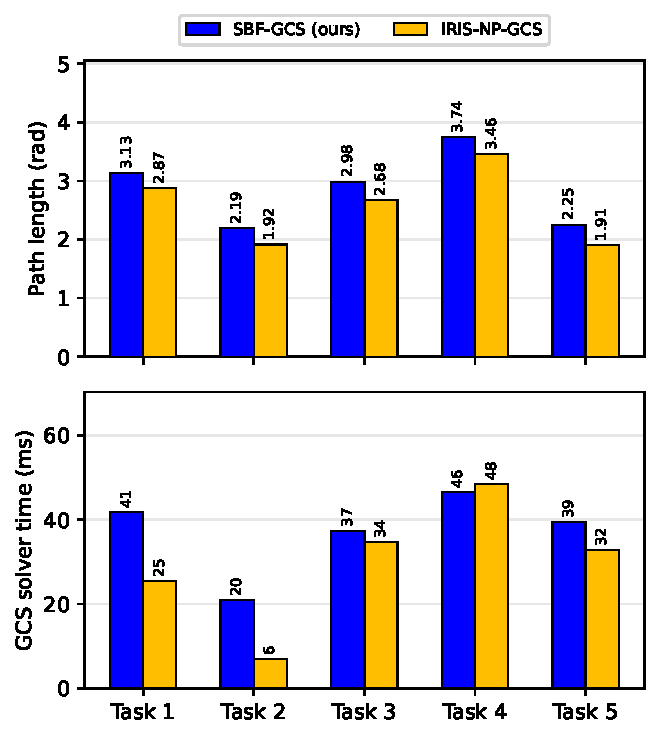
\includegraphics[width=\columnwidth]{fig/fig_exp2_bars.pdf}
\caption{Per-pair GCS planning results.
  Top: C-space path length~(rad); bottom: GCS solver time~(ms).
  SBF-GCS achieves 98\% success (49/50) vs.\ IRIS-NP-GCS 100\%.
  SBF: 10~seeds; IRIS-NP: 10~repeats.}
\label{fig:exp2}
\end{figure}

\emph{Analysis.}
SBF-GCS achieves a 98\% overall success rate (49/50 query--seed
combinations) versus 100\% for IRIS-NP-GCS (\cref{fig:exp2}).
Despite SBF's lower global coverage (24\% vs.\ 60\%,
\cref{tab:exp1}), the densely packed boxes concentrate certified
regions along planning-relevant corridors, preserving connectivity
for nearly all queries (\cref{fig:exp2_viz}).
SBF path lengths are on average 11\% longer than IRIS-NP
(mean 2.86\,rad vs.\ 2.57\,rad across all tasks), reflecting the finer
granularity of hyperrectangular regions compared to large polytopes.
The gap is smallest on Task~4 (8\%, the hardest long-detour pair) and
largest on Task~5 (18\%).
GCS solver times are comparable: SBF averages 37.2\,ms vs.\ IRIS-NP
29.7\,ms, and SBF is even slightly faster on Task~4
(46.5\,ms vs.\ 48.5\,ms) despite its larger graph
(${\sim}$885 nodes vs.\ 8).
Both methods' solver times remain in the tens-of-milliseconds range,
negligible compared to region generation
(SBF: ${\sim}$1\,s; IRIS-NP: ${\sim}$90\,s).
The single failure arises from a connectivity gap in the box forest for
one random seed; this is addressable by increasing the random-fill budget
or bridge-paving effort.

% ──── Exp 3 ──────────────────────────────────────────────────────────────────
\subsection{Incremental Update}\label{sec:exp3}

Starting from a fully constructed forest, we randomly select one
bin or shelf obstacle and apply a 5\,cm random translation.
This simulates a typical single-object perturbation in manipulation
tasks.
Each seed undergoes 10 consecutive perturbation trials
(100 trials total across 10 seeds).
We compare three reconstruction strategies:
\emph{incremental} (targeted regrow: invalidation $+$
\texttt{regrow($2 n_\text{inv}$)}),
\emph{warm rebuild} (invalidation $+$ full \texttt{build\_multi}
reusing the FK cache), and
\emph{cold rebuild} (fresh planner, no prior cache).

\begin{table}[t]
\centering
\caption{Incremental update vs.\ warm/cold rebuild after 5\,cm
  single-obstacle perturbation (100 trials, 10 seeds $\times$ 10).}
\label{tab:exp3}
\footnotesize
\begin{tabular}{@{}lccc@{}}
\toprule
  & Incremental & Warm & Cold \\
\midrule
Time (median) & \textbf{7\,ms} & 727\,ms & 1{,}059\,ms \\
Time (mean)   & \textbf{11\,ms} & 775\,ms & 1{,}134\,ms \\
Boxes (median) & 916 & 854 & 854 \\
Volume ($\text{rad}^7$, median) & 5.82 & 8.98 & 8.98 \\
Invalidated (med.) & 90 & --- & --- \\
\midrule
Fraction of cold time & \textbf{1/150} & 1/1.53 & 1 \\
Vol.\ ratio (vs.\ cold) & 0.65 & 1.0 & 1.0 \\
\bottomrule
\end{tabular}
\end{table}



\emph{Analysis.}
A single-obstacle 5\,cm perturbation invalidates $\sim$90~boxes
($\sim$10\% of the forest).
Targeted regrow refills these gaps in $\textbf{7}$\,\textbf{ms}~(median).
This is only \textbf{1/150} of the cold-rebuild time
($7$\,ms vs.\ $1.06$\,s) and \textbf{1/104} of warm-rebuild time
($7$\,ms vs.\ $0.73$\,s).
The regrown forest contains slightly more boxes (916 vs.\ 854)
because coarsening is skipped.
The resulting volume is 65\% of cold-rebuild volume.
This is a reasonable tradeoff given the two-orders-of-magnitude
speed gain.
Warm rebuild re-executes the full construction pipeline with FK-cache
reuse.
It achieves only $1.53\times$ speedup over cold, confirming that the
bottleneck lies in the pipeline stages rather than FK computation.
IRIS-NP provides no built-in mechanism for incremental updates.
In practice, any scene change requires discarding and regrowing all
regions from scratch ($\sim$90\,s).
SBF's $7$\,ms incremental update is four orders of magnitude
faster than this full-rebuild baseline.

% ==============================================================================
% VI. CONCLUSION
% ==============================================================================
\section{Conclusion}\label{sec:conclusion}

We presented SafeBoxForest, a certified region generator for GCS
motion planning backed by a lazy lifelong AABB cache.
The LECT lazily maps C-space boxes to certified
workspace AABB envelopes via interval-FK.
Each envelope is computed on demand when first queried and cached
permanently.
Because envelopes depend only on robot kinematics, the cache is
reusable for the robot's entire lifetime.
Given a specific obstacle scene, SBF queries the LECT and grows a
collision-free box forest via RRT-like wavefront expansion.
Greedy coarsening merges fine boxes into hundreds of certified regions.
The resulting forest maps directly to a GCS graph.
SBF achieves competitive planning performance
(98\% success rate, paths only 11\% longer than IRIS-NP on average)
with region generation $86$--$123\times$ faster than IRIS-NP.
SBF also provides formal safety guarantees that IRIS-NP lacks.
The LECT cache and targeted regrowth transform region generation
from ``rebuild every time'' to ``incremental maintenance.''
Regrowth requires only $1/150$ of cold-rebuild time
($7$\,ms vs.\ $1.06$\,s) for single-obstacle updates.
All safety guarantees are conditioned on \cref{asm:geom} and the
AABB obstacle model; violations of either assumption void the
certificate.

\textbf{Limitations.}
Hyperrectangles yield lower per-region volume than polytopes
(24\% vs.\ 60\% global coverage), though dense packing preserves
a 98\% success rate.
The method assumes serial DH kinematics and AABB obstacles;
for $D>7$ the interval wrapping effect progressively loosens envelopes.
Evaluation is limited to a single platform (KUKA IIWA14).

\textbf{Future work.}
OBB envelopes or affine arithmetic could tighten enclosures and
mitigate wrapping.
Hybrid SBF--IRIS approaches, adaptive subdivision depth, and
multi-core wavefront parallelization are promising extensions.
Evaluation on additional manipulators and obstacle geometries
remains an important direction.

% ==============================================================================
% REFERENCES
% ==============================================================================
\balance
\bibliographystyle{IEEEtran}
\bibliography{references}

\end{document}
